\documentclass[12pt,a4paper,Flow]{report}
\usepackage[left=1.8cm,right=1.8cm,top=2cm,bottom=1.5cm]{geometry}
\usepackage[BoldFont]{xeCJK}
\usepackage{xeCJK}
\usepackage{graphicx}
\usepackage{float}
\usepackage{indentfirst}
\usepackage{fancyhdr}
\usepackage[toc,header,title]{appendix}
\usepackage{color,xcolor}
\usepackage{listings}
\usepackage{tikz}
\defaultfontfeatures{Mapping=tex-text}
\definecolor{llgray}{rgb}{0.9,0.9,0.9}
\lstloadlanguages{python}
\lstset{
  language=python,tabsize=4,keepspaces=true,
  xleftmargin=2em,xrightmargin=2em,aboveskip=1em,
  frame=none,
  commentstyle=\color{red}\itshape, % blue comments
  keywordstyle=\color{blue}\bfseries,
  backgroundcolor=\color{llgray},
  breakindent=22pt,
  numbers=left,stepnumber=1,numberstyle=\tiny,
  basicstyle=\footnotesize,
  showspaces=false,
  showstringspaces=false, % show explicit string spaces
  flexiblecolumns=false,%true,
  breaklines=true,breakautoindent=true,breakindent=4em,
  escapeinside={/*@}{@*/}
}
\usepackage[a4paper,CJKbookmarks,bookmarks=true,bookmarksopen=true]{hyperref}%很强大的一个东西
\hypersetup{
  pdftitle={},
  pdfauthor={Wang Pei},
  pdfkeywords={},
  bookmarksnumbered,
  breaklinks=true,
  pdfview=FitV,       % Or try pdfstartview={FitV}, This lead to uncorre
  urlcolor=cyan,
  colorlinks=true,
  citecolor=magenta,          %citeref's color
 linkcolor=blue,
}
\usepackage{titlesec}
\titleformat{\chapter}{\centering\huge}{\textbf{第}\thechapter{} \textbf{章}}{1em}{\textbf}

\renewcommand\contentsname{目录}
\renewcommand{\appendixpagename}{附录}
\renewcommand{\appendixname}{附录}

\setmainfont{DejaVu Sans}
\setCJKmainfont[BoldFont=WenQuanYi Micro Hei]{SimSun}

\begin{document}
  \title{\textbf{体系结构实习——UniCore2模拟器\\实习报告}}
  \author{张番栋 00848180\\刘澜涛 00848200\\王 沛 00848205\\CS08}
  \date{\today}
  \maketitle
  \tableofcontents
  \newpage
  \chapter{实习内容}
  \section{目标}
  实习的主要内容是用C语言编写一个支持UniCore2精简指令系统的模拟器,并对其进行测试、验证。在之后的报告中,均称实习所完成的模拟器为MinSim。MiniSim的首要目标是进行正确的功能模拟,在此基础上增加对CPU流水线以及Cache的结构模拟,另外还有对程序动态运行情况的统计。MiniSim采用五级流水结构,和真实的UniCore2处理器并不相同。模拟的Cache则具有较灵活的定制性。\\
  \section{具体实现功能}
  \indent MiniSim支持的UniCore2指令子集中包含五类指令:
  \begin{itemize}
  \item 数据处理指令
  \item 乘法和乘加指令
  \item 跳转切换指令
  \item 单数据传输指令
  \item 条件转移指令和带链接条件转移指令。
  \end{itemize}
  \indent 从中可以看出,MiniSim并未对处理器特权状态的相关功能进行模拟,进而无法完全支持基于现代操作系统下的大部分程序。针对这个问题,我们做了一些工作,使得MiniSim在接受标准ELF文件作为输入的情况下,仍然能够完成大部分应用级别的功能模拟。\\
  \indent 本次实习是与编译实习联合进行,因此我们在完成实习的过程中做了一些编译器和模拟器之间的协调工作。\\
  \indent 最后,为了方便使用和调试,我们为MiniSim编写了一个简单的控制台模块,使得MiniSim在运行时可以设置断点,单步执行、查看寄存器、内存和流水线的状态。
  \chapter{模拟器详解}
  \section{模拟器的内存管理}
  MiniSim在运行时需要在自己的地址空间内同时维护目标程序的地址空间,因此需要建立一套面向目标程序的虚拟内存机制。在这个问题上,MiniSim采用的是页式内存管理机制。对于目标程序的32位地址空间,MiniSim进行了如下划分
  \begin{itemize}
  \item 31-25 位: 一级页表偏移
  \item 24-15 位: 二级页表偏移
  \item 14-0 位: 页内偏移
  \end{itemize}
  \begin{figure}[H]
    \centering
    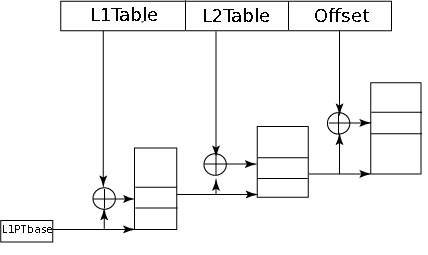
\includegraphics[width=0.5\textwidth]{pt.png}
  \end{figure}
  也就是说,页的大小为32KB。一级页表常驻内存,共有128个页表项,每个页表项大小为4B,即指向二级页表的指针。每个二级页表含有1024个页表项,每个页表项8B,存储的信息包括其所指向的页的起始地址和该页的读、写、执行属性。\\
  \indent 这是一个很经典的虚拟内存管理机制,尤其在管理目标程序的栈时可以提供较好的局部性。在这种机制下,只要模拟器的存储管理模块要提供读、写内存的操作接口,真正执行目标程序的模块就可以减少很多工作量。同时,页式结构在一定程度上可以对非法的内存访问做一些检测。
  \section{模拟器运行环境的建立}
  MiniSim接受标准ELF文件作为输入。在真正模拟运行目标机程序之前,需要做一些初始化工作。换言之,MiniSim需要完成一部分装载器和操作系统的工作。主要内容有ELF文件解析
内存环境的建立、代码段和数据段的载入、寄存器堆和流水线的初始化等等。
  \subsection{对系统相关指令、功能的处理}
  由于MiniSim不支持操作系统级别的指令,同时也不需要支持复杂的程序运行环境,所以模拟区间仅限于main函数。也就是说,MiniSim会跳过main函数之前的代码段,待main函数结束后退出。另外,为了便于检查,MiniSim还需要支持整型数据的非格式化输出。输出是与系统调用有关的功能,因此需要做一些约定:在给予MiniSim的输入中,输出功能要被封装在一个特定的函数中。当模拟进行到这个函数时,模拟器会以宿主机的输出调用替代之,然后结束该函数,从返回地址继续执行。为了达到这个目的,需要在ELF文件装载阶段进行一些工作。
  \subsection{ELF文件解析}
  需要做的工作主要有两点:
  \begin{enumerate}
  \item 获取main和输出封装函数的入口地址。
  \item 获得ELF文件中代码段和数据段的位置和大小,以备建立模拟内存环境之用。
  \end{enumerate}
  具体的
  \subsection{寄存器堆和流水线初始化}
  
\end{document}
